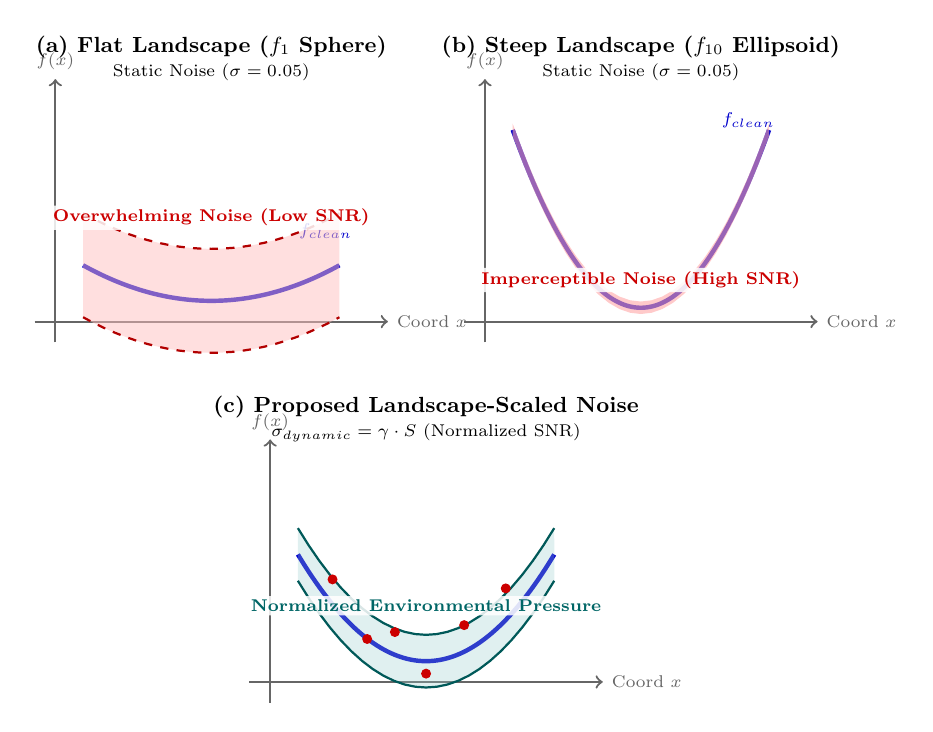
\begin{tikzpicture}[scale=0.88, every node/.style={transform shape}]

    % Style for text labels inside plot areas to prevent lines crossing text
    \tikzset{
        labelmask/.style={fill=white, fill opacity=0.85, text opacity=1, inner sep=1.5pt, rounded corners=1pt, font=\scriptsize}
    }

    % -------------------------------------------------------------------------
    % Subfigure A: Flat Function with Static Noise
    % -------------------------------------------------------------------------
    \begin{scope}[shift={(0,0)}]
        \draw[->, thick, gray!80!black] (-0.3,0) -- (4.8,0) node[right, font=\scriptsize] {Coord $x$};
        \draw[->, thick, gray!80!black] (0,-0.3) -- (0,3.5) node[above, font=\scriptsize] {$f(x)$};
        
        \node[font=\bfseries\small, align=center] at (2.25, 3.8) {(a) Flat Landscape ($f_1$ Sphere)\\[-1pt]\normalfont\scriptsize Static Noise ($\sigma=0.05$)};
        
        % Clean Curve
        \draw[blue!80!black, ultra thick, domain=0.4:4.1, samples=100] plot (\x, {0.15*(\x-2.25)^2 + 0.3});
        \node[blue!80!black, font=\bfseries\scriptsize] at (3.9, 1.3) {$f_{\text{clean}}$};
        
        % Overwhelming Noise Envelope
        \fill[red!25, opacity=0.5, domain=0.4:4.1] 
            plot (\x, {0.15*(\x-2.25)^2 + 0.3 + 0.75}) -- 
            plot[domain=4.1:0.4] (\x, {0.15*(\x-2.25)^2 + 0.3 - 0.75}) -- cycle;
        \draw[red!70!black, dashed, thick, domain=0.4:4.1] plot (\x, {0.15*(\x-2.25)^2 + 0.3 + 0.75});
        \draw[red!70!black, dashed, thick, domain=0.4:4.1] plot (\x, {0.15*(\x-2.25)^2 + 0.3 - 0.75});
        
        \node[labelmask, text=red!80!black, font=\bfseries\scriptsize] at (2.25, 1.5) {Overwhelming Noise (Low SNR)};
    \end{scope}

    % -------------------------------------------------------------------------
    % Subfigure B: Steep Function with Static Noise
    % -------------------------------------------------------------------------
    \begin{scope}[shift={(6.2,0)}]
        \draw[->, thick, gray!80!black] (-0.3,0) -- (4.8,0) node[right, font=\scriptsize] {Coord $x$};
        \draw[->, thick, gray!80!black] (0,-0.3) -- (0,3.5) node[above, font=\scriptsize] {$f(x)$};
        
        \node[font=\bfseries\small, align=center] at (2.25, 3.8) {(b) Steep Landscape ($f_{10}$ Ellipsoid)\\[-1pt]\normalfont\scriptsize Static Noise ($\sigma=0.05$)};
        
        % Clean Curve
        \draw[blue!80!black, ultra thick, domain=0.4:4.1, samples=100] plot (\x, {0.75*(\x-2.25)^2 + 0.2});
        \node[blue!80!black, font=\bfseries\scriptsize] at (3.8, 2.9) {$f_{\text{clean}}$};
        
        % Tiny Static Noise Envelope
        \fill[red!35, opacity=0.6, domain=0.4:4.1] 
            plot (\x, {0.75*(\x-2.25)^2 + 0.2 + 0.09}) -- 
            plot[domain=4.1:0.4] (\x, {0.75*(\x-2.25)^2 + 0.2 - 0.09}) -- cycle;
            
        \node[labelmask, text=red!80!black, font=\bfseries\scriptsize] at (2.25, 0.6) {Imperceptible Noise (High SNR)};
    \end{scope}

    % -------------------------------------------------------------------------
    % Subfigure C: Landscape-Scaled Noise (Normalized SNR)
    % -------------------------------------------------------------------------
    \begin{scope}[shift={(3.1,-5.2)}]
        \draw[->, thick, gray!80!black] (-0.3,0) -- (4.8,0) node[right, font=\scriptsize] {Coord $x$};
        \draw[->, thick, gray!80!black] (0,-0.3) -- (0,3.5) node[above, font=\scriptsize] {$f(x)$};
        
        \node[font=\bfseries\small, align=center] at (2.25, 3.8) {(c) Proposed Landscape-Scaled Noise\\[-1pt]\normalfont\scriptsize $\sigma_{\text{dynamic}} = \gamma \cdot S$ (Normalized SNR)};
        
        % Clean Curve
        \draw[blue!80!black, ultra thick, domain=0.4:4.1, samples=100] plot (\x, {0.45*(\x-2.25)^2 + 0.3});
        
        % Proportional Landscape Noise Envelope
        \fill[teal!40, opacity=0.3, domain=0.4:4.1] 
            plot (\x, {0.45*(\x-2.25)^2 + 0.3 + 0.38}) -- 
            plot[domain=4.1:0.4] (\x, {0.45*(\x-2.25)^2 + 0.3 - 0.38}) -- cycle;
        \draw[teal!70!black, thick, domain=0.4:4.1] plot (\x, {0.45*(\x-2.25)^2 + 0.3 + 0.38});
        \draw[teal!70!black, thick, domain=0.4:4.1] plot (\x, {0.45*(\x-2.25)^2 + 0.3 - 0.38});
        
        % Sample Noisy Points
        \filldraw[red!80!black] (0.9, 1.48) circle (1.8pt);
        \filldraw[red!80!black] (1.4, 0.62) circle (1.8pt);
        \filldraw[red!80!black] (1.8, 0.72) circle (1.8pt);
        \filldraw[red!80!black] (2.25, 0.12) circle (1.8pt);
        \filldraw[red!80!black] (2.8, 0.82) circle (1.8pt);
        \filldraw[red!80!black] (3.4, 1.35) circle (1.8pt);
        
        \node[labelmask, text=teal!80!black, font=\bfseries\scriptsize] at (2.25, 1.1) {Normalized Environmental Pressure};
    \end{scope}

\end{tikzpicture}